\section{Background}
\label{section:background}

In this section we will review basics of the video broadcasting protocols,
modulation algorithms, error correction schemes, video encapsulation 
formats, audio and video codecs, as well as security mechanisms, which are
needed for protection of video streams from eavesdropping by malicious parties.

\subsection{DVB standards}

Today there exist three major standards which are used for delivering 
live video content to customers: digital video broadcast 
over cable (DVB-C), terrestrial digital video broadcast (DVB-T), and
digital video broadcast over satellite (DVB-S). We will review these 
standards, as well as their modifications, so-called second generation
broadcasting protocols, in the given section.

{\bf DVB-C}

{\bf DVB-T}

{\bf DVB-S}

{\bf Second generation digital video broadcast protocols}

\subsection{Modulations}

On high level an information signal, before being transmitted over the medium, such as cable
or air, needs to be modulated (combined with carrier frequency) in some way. 
There exist multiple modulation schemes, examples are frequency modulation, amplitude
modulation, phase modulation, and their combinations. In this section, in addition to already 
mentioned, we will review two additional modulation 
schemes: quadrature phase shift keying modulation (QPSK) 
and quadrature amplitude modulation (QAM).

The most simple modulation is \textit{amplitude modulation}. It can be 
described in the following manner. If the carrier
signal is represented as $c(t) = A_c\sin(2\pi f_ct)$, where $A_c$ is the 
peak value of amplitude of the carrier, $f_c$ is the carrier
frequency and $t$ is time; and the modulating signal is represented
as $m(t)=A_m\sin(2\pi f_mt)$, where the $A_m$ is the peak value of the amplitude of the 
modulating signal, $f_m$ is the modulating frequency, then
the modulated signal can be described as  
$y(t) = (A_c + A_m \sin(2\pi f_mt))\sin(2\pi f_ct) = A_c(1+M \frac{1}{A_m}m(t))c(t)$, 
where $M= \frac{A_m}{A_c}$ is the modulation index.
Simplifying\footnote{http://www.tofmal.ru/projects/trigan/page5.html} the equation 
we get $y(t) = A_c\sin(2\pi f_ct) + \frac{A_cM}{2}cos(2\pi(f_c-f_m)t) - 
\frac{A_cM}{2}cos(2\pi(f_c+f_m)t)$, in other words the modulated signal 
(for single tone modulating signal) consists of three harmonics: 
central frequency, and two side-bands. In Figure~\ref{fig:am} we show how 
amplitude modulated signal will look like when a single tone modulating signal 
(with frequency equal to $2$Hz) is combined with $100$Hz carrier signal. 
The sidebands in this case will be signal with frequency $98$Hz and 
signal with frequency $102$Hz.
Now coming back to the modulation index: typically, it should be 
well above the zero, but also less than or equal to one. A modulation index larger than one indicates 
the over-modulation situation. Such signal cannot be demodulated and therefore no
intelligence can be recovered from it. The ideal condition is when $A_c = A_m$, which gives $100\%$ modulation. 
This situation results in the greatest output power at the transmitter and the greatest output
voltage at the receiver, with no distortion~\cite{}. 

\begin{figure}[ht]
\includegraphics[width=0.5\textwidth]{graphics/microbanchmarking/amplitude_modulation.pdf}
\caption{Amplitude modulation}
\label{fig:am}
\end{figure}

Other simple examples of modulation are Amplitude Shift Keying (ASK)
and On-Off Keying (OOK). In amplitude shift keying only single 
carrier frequency is present, but the amplitude is changed from time
to time. With this modulation it is easy to encode 
binary message: a signal with high amplitude represents the binary
1, and signal with low amplitude represents binary 0. In on off keying
modulation is achieved by simply turning the carrier on and off. Example
of such modulation is Morse code: the dot is represented with a short
burst of carrier, and dash is modulated with long burst of carrier 
signal. Code transmission such as this are usually called 
\textit{continuous-wave (CW) transmissions}. 

In frequency modulation the frequency is modified for the purpose of transmission
of intelligence signal. Unlike the amplitude modulation, in frequency modulation
the amplitude remains constant and only the frequency of the carrier is being 
changed. In frequency modulation the carrier frequency changes proportional to 
the changes of the voltage of the intelligence signal: that is, as the 
modulating signal voltage increases, the carrier frequency also increases;
as the modulating signal's voltage decreases, the carrier frequency also 
decreases.

Another way to modulate signals is to shift the phase of the carrier signal
depending on the values of the intelligence signal. These modulations are known as 
phase shift keying (or PSK). Examples are Binary Phase Shift Keying, Quadrature Phase
Shift Keying (QPSK) and Quadrature Amplitude Modulation. It is perhaps easier to understand these 
modulations with the following example. Lets consider a phase modulated signal $y(t) = A \cos(2\pi f_c t + \varphi)$. 
Using trigonometric identity\footnote{www.ni.com/tutorial/4805/en/} we can derive 
$A\cos(2\pi f_c t + \varphi) = A\cos(2\pi f_c t) \cos(\varphi) - A \sin(2\pi f_c t)\sin(\varphi)$.
Now substituting $I(t) = A \cos(\varphi)$ and $Q(t) = A \sin(\varphi)$, we 
get $A\cos(2\pi f_c t + \varphi) = I(t) \cos(2\pi f_c t) - Q(t) \sin(2\pi f_c t)$.
Here $I(t)$ represents the in-phase part of the signal, $Q(t)$ represents the quadrature 
part of a signal. By carefully selecting $A=\sqrt{2}$ (knowing that 
$\varphi \in \{\frac{\pi}{4}, \frac{3\pi}{4}, \frac{5\pi}{4}, \frac{7\pi}{4}\}$), 
$I(t)$ and $Q(t)$ will take values $\{-1, 1\}$. This can be easily seen from IQ diagrams 
(also called constellation diagram, or phasor diagram), which we show in 
Figure~\ref{fig:constellation}. So, for example, if we need to encode the binary message \texttt{00},
the resulting signal can be described with the following equation $y(t) = I(t)\cos(2\pi f_c t) - Q(t)\sin(2\pi f_c t) = 
\cos(2\pi f_c t) - \sin(2\pi f_c t)$. The signal will have $\frac{\pi}{4}$ phase shift
relative to in-phase signal (see Figure~\ref{fig:iqexample} for reference).

\begin{figure}[ht]
\centering
\includegraphics[width=0.3\textwidth]{graphics/constellation.png}
\caption{Constellation diagram}
\label{fig:constellation}
\end{figure}

\begin{figure}[ht]
\centering
\includegraphics[width=0.5\textwidth]{graphics/iq.pdf}
\caption{Example of IQ signal}
\label{fig:iqexample}
\end{figure}

In Figure~\ref{fig:qpsk}, we show how the binary message \texttt{00 01 11 10} will 
be modulated using $5$Hz carrier signal. 

\begin{figure}[ht]
\centering
\includegraphics[width=0.5\textwidth]{graphics/qpsk.pdf}
\caption{Modulation of \texttt{00 01 11 10} binary message}
\label{fig:qpsk}
\end{figure}

To perform demodulation, modulated signal should be multiplied by $cos(2\pi f_c t)$ to obtain 
the $I(t)$ component, and by $-sin(2\pi f_c t)$ to obtain the $Q(t)$ component of the signal. 
Both signals then should be passed through low-pass filter (or exponentially weighted moving average function) 
so that the original binary message can be recovered (the values of $I(t)$ and $Q(t)$ will be selected based 
on the sign of a sample at time $t$: that is, if the value of a sample is greater than $0$, $I(t)$ or $Q(t)$ will be $1$, 
otherwise $-1$ will be assigned to $I(t)$ or $Q(t)$). In Figure~\ref{fig:qpsk_demodulated} we demonstrate the demodulated 
$I(t)$ and $Q(t)$ values for previously modulated message - \texttt{00 01 11 10}. 

There are other variants of PSK. To name a few, we can mention Binary Phase Shift 
Keying (which can encode one bit per symbol) and 
Quadrature Amplitude Modulation (16-, 64-, 256-QAM). With latter one, 
$4$, $6$, and $8$ bits per symbol can be transmitted. In QAM the idea is basically
the same as in QPSK, whereas the difference lies in the constellation diagram: there are
many points per quarter (for example, in 16-QAM there are 4 such points). To decrease
the bit error rate (BER) grey code is used to represent the values in 
constellation diagram. Finally, we should note that DVB-C uses variants of 
QAM modulation (typically 16-, 64- and 256-QAM is being used).

\begin{figure}[ht]
\centering
\includegraphics[width=0.5\textwidth]{graphics/qpsk_demod_lowpass.pdf}
\caption{Decoding binary message}
\label{fig:qpsk_demodulated}
\end{figure}

%{\bf A note on mathematical background}

%{\bf OFDM} modulation

%{\bf QPSK} modulation

%{\bf QAM} modulation

\subsection{Error correction}

A signal, when transmitted over the medium, can be distorted 
in many ways (for example, due to radio signal attenuation, interference, 
reflection and other physical phenomena). This will undoubtedly lead 
to corruption of information. Therefore, it is typically 
needed to embed some redundant information into the transmitted message, 
so that the recipient can recover the original message even if some 
information is corrupted or lost. One such algorithm is Reed-Solomon 
forward error correction (or FEC). We will review its basics in this 
section.

{\bf Reed Solomon} error correction algorithm.

\subsection{MPEG standards}

{\bf MPEG-2} standard defines how to format the various component parts of a 
multimedia program. The program may consist of several parts, including 
compressed MPEG-2 video, compressed audio, control and user data. It 
also defines how these components are combined into single synchronous 
transmission bit stream~\cite{mpegts}. The process of combining is known 
as {\it multiplexing}. 

\begin{figure*}[ht]
\includegraphics[width=1\textwidth]{graphics/ts_packet.png}
\caption{Transport stream packet structure}
\label{fig:ts_packet}
\end{figure*}

{\bf MPEG transport stream}. MPEG-TS, which is defined in ISO/IEC 13818-1, 
is essentially a stream of packets containing encoded multimedia and control data.
All packets belong to some elementary stream. MPEG transport stream consists of
a sequence of packets of one or more elementary streams multiplexed into 
one common stream. All packets, as we will discuss later, have an identifier
which indicates to which elementary stream the packet belongs.

Each MPEG-TS packet contains a header and a usable payload, such as audio, 
video information and control data. The structure of a typical MPEG-TS 
packet is shown in Figure~\ref{fig:ts_packet}. The entire size of a MPEG-TS packet 
is just $188$ bytes. The header size is $4$ bytes and carries important 
information about the payload, leaving only $184$ bytes (or less, depending 
on whether an adaption header is present or not) to the actual payload. 
The transport stream packet starts with a synchronization byte, whose 
value should be \texttt{0x47} in hexadecimal notation. This byte is 
recognized by the decoder so that the header and the payload can be 
deserialized. Next follows the transport error indicator (TEI) bit, 
which, if set to $1$, signalizes that the packet has an error and should 
be discarded. The next bit is the payload unit start indicator (PUSI). 
If the bit is set, then it means that the packet is the start of a new 
packetized elementary stream (PES). Otherwise, it is a continuation 
of an existing PES. As a side note, we should mention that elementary 
streams can be of two types: (i) packetized elementary stream, which 
carries video, audio or subtitles and can be up to $65536$ bytes
long, or (ii) sections, i.e., data structures. The last TS packet for PES packet
will contain adaptation header with enough \textit{stuffing} bytes so that end of PES
will match the end of TS packet. Next bit, following PUSI bit, is the transport priority
(TP) bit, which gives the packet high priority over the packets with the same
packet identifier (discussed next). More important (in the course of this work) 
is the next $13$ bits sequence, which encodes unique packet identifier, 
or PID. A PID can have $8192$ unique values, which corresponds to a maximum 
number of independent elementary streams.
%A MPEG-TS can be multiple or single program multimedia stream. 
%For a single multimedia stream, apart from control packets, there can
%be just two types of elementary streams: one for video packets, and one for 
%audio packets, each identified with a unique PID. As we have already mentioned
%even a single multimedia stream may contain elementary streams other
%than audio and video.

Some predefined values for PIDs are listed in Table~\ref{tab:pids}. 
An elementary stream is a sequence (concatenation) of transport stream packets 
with the same PID value in the header. Thus, for example, the video elementary 
stream for a certain program will always have the same PID. This can be used
to efficiently demultiplex the program. Next $2$ bits carry information about 
scrambling (encryption) of payload. This two-bit sequence is denoted as 
scrambling control (SC). Adaption Field Control (AFC) is a two bits 
sequence. A thorough description of this field and the actual adaptation field 
can be found in~\cite{MPEG2:overview}. The last field in the header 
is the continuation counter (CC). The counter can have $16$ values and
is used to detect loss, reordering, and duplicates. 

The two most important PIDs (not taking into consideration the PIDs for 
actual audio and video packets) are \texttt{0x00} for the program association table (PAT)
and the PID for program map table (PMT). The PID for the program map table can be found
in the program association table. In turn, the PIDs for audio and video data can be 
found program map table. As indicated in~\cite{dtv}, PAT and PMT are transmitted at
a maximum interval of $500$ms.

%Therefore, one elementary stream contains one single
%type of content: audio for one language, video, subtitles for one language,
%exception as a text, etc.

\begin{table}
 \caption{Common packet identifiers}
\begin{tabular}{|l|l|}
  \hline
 PID (hex)                        & Description                                                      \\
  \hline
  \texttt{0x00}                   & PAT, Program Association Table                                   \\
  \texttt{0x10}                   & NIT, Network Information Table                                   \\
  \texttt{0x11}                   & BAT, Bouquet Association Table                                   \\
  \texttt{0x11}                   & SDT, Service Descriptor Table                                    \\
  \texttt{0x12}                   & EIT, Event Information Table                                     \\
  \texttt{0x13}                   & RST, Running Status Table                                        \\
  \texttt{0x14}                   & TOT, Time Offset Table                                           \\
  \texttt{0x20} - \texttt{0x1FFA} & PMT, Program Map Table, other elementary streams                 \\
  \texttt{0x1FFF}                 & Null packet                                                      \\
  \hline
\end{tabular}
\label{tab:pids}
\end{table}

{\bf Audio and video codecs}. Most common video codec found in MPEG-2 
standard is H.264~\cite{}. For audio AAC audio codec is being tipically
used~\cite{} in MPEG-TS streams. In this section we will briefly review 
these codecs, while a thorough description can be found in~\cite{}.

\subsection{HTTP Live Streaming (HLS)} 
The details of HLS protocol are described in RFC 8216~\cite{rfc8216}.
Here we will briefly outline its key concepts.

\subsection{Security}

Digital restrictions management (DRM) is essential in digital era. Briefly, 
it can be described as a set of practices and techniques used to protect 
the content from unauthorized viewing and distribution. There are 
perhaps many solutions to protect the content from being eavesdropped, 
but in this work, we will focus only on encryption of streams 
with block ciphers. HLS and DVB use different 
approaches (in terms of algorithms) to protect the video streams from 
unauthorized usage. Thus, in HLS the entire MPEG-TS stream is encrypted 
with the widely used Advanced Encryption Standard (AES) algorithm~\cite{Stinson:Cryptography}, 
using a key of size $128$ bits. DVB, in turn, uses its own, or shall we 
say domain specific, block cipher called the Common Scrambling Algorithm 
(CSA)~\cite{breakingdvbcsa}, with a relatively small key of just $48$ bits 
in length (in reality, the key is equal to block size, but the $2$ bytes in the 
key are computed in a deterministic manner, leaving only $48$ bits of 
entropy). 

{\bf DVB Common Scrambling Algorithm (DVB-CSA)} is a proprietary 
algorithm, which was designed for DVB standards. In essence, CSA
is a block cipher, which operates in two phases. In the first 
phase, the payload is split into equal size blocks, each of size $64$ bits.
All blocks are then encrypted in reverse order: the first block in order 
(the last block in the original sequence) is encrypted using all zero 
initialization vector, all other blocks prior to encryption are also 
xored with the previously encrypted block (here block cipher is also initialized
with all zero initialization vector). The first block in the original sequence 
is also tweaked with an encryption key. In the second phase, each block, starting
from the second block (in original order), is \textit{xored} with the key: the key for the second pass 
is produced with a stream cipher, which is initialized with the value of the first block 
and the encryption key. In Figure~\ref{fig:dvbcsa} we schematically demonstrate 
the operation of CSA algorithm. 
%Unlike AES symmetric key algorithm, in which blocks are of size $128$ 
%bits, in CSA the blocks have length of $64$ bits. 

\begin{figure}[ht]
\includegraphics[width=0.45\textwidth]{graphics/csa_arch.png}
\caption{DVB-CSA structure}
\label{fig:dvbcsa}
\end{figure}

{\bf HLS security}. As described in ~\cite{rfc8216}, the media segments
can be delivered as plaintext (with no encryption), encrypted with AES-128 
in Cipher Block Chaining (CBC) mode~\cite{Stinson:Cryptography}, or as ciphertext
produced with SAMPLE-AES encryption method. 

As the name implies, in no encryption mode nothing is being encrypted and
segments are delivered to clients as a plaintext. Of course,
HTTP supports secure mode of operation, which is known as HTTPS. 
Secure version is built with help of SSL~\cite{rfc6101} or TLS~\cite{rfc5246} protocol. 
This means that eavesdropper will not be able to get access to contents of 
segments, even if it will sniff packets on wire or air. 
However, additional mechanisms for authentication and authorization 
are still required to protect segments from unauthorized access.

If HLS implements encryption with AES method, then entire segments are encrypted 
using AES encryption in CBC mode using $128$ bit key. When this approach is implemented, 
EXT-X-KEY attribute in the playlist file must specify 
appropriate encryption method (see for reference~\cite{rfc8216}), URL 
of the key file, block cipher initialization vector (IV),
and some other parameters. It is then responsibility of the client 
to decrypt the segments using appropriate parameters.
We should note that key can be protected from unauthorized access with cookie 
files~\cite{httpcookie}. This means that the client first needs to use methods advertised 
by the content provider to authenticate itself, and only then try to access encrypted 
segments and key file. It is rather arguable whether this mechanism is more  
advantageous over mechanism with no encryption when used together with HTTPS protocol. 
On one hand, one can build a similar access mechanism for plaintext segments, 
i.e., the delivery of segments can be organized over HTTPS protocol, while cookies
can be used for authentication. On the other hand, when AES mode of encryption is being used together with 
HLS protocol, the need for HTTPS to deliver the media segments vanishes (segments 
can be securely delivered over insecure HTTP protocol, and only key file needs to 
be transmitted over encrypted tunnel). This means that extra CPU cycles, which are
needed to perform key exchange, key derivation and encryption of the payload, 
can be avoided. Perhaps, real-life measurements can shed a light on this matter.

Finally, there is SAMPLE-AES method. In this method, only  
media samples such as audio or video, contained in segments, 
are encrypted using AES algorithm. How this media segments 
are encrypted and encapsulated depends largely on media 
encoding~\cite{rfc8216}.


